\documentclass[a4paper]{article}

\usepackage{fullpage}
\usepackage{setspace}
\usepackage{url}
\usepackage{algorithmic}
\usepackage{algorithm}
\usepackage{amsmath}
\usepackage{latexsym}

\usepackage{graphicx}
\usepackage{subfig}

\onehalfspacing

\newtheorem{definition}{Definition}
\newtheorem{theorem}{Theorem}
\newtheorem{example}{Example}
\newtheorem{query}{Query}

\newcommand{\nop}[1]{}

\title{Mapping Microblogging Posts to Encyclopedia Articles}
\author{David M\"{u}ller \and Uta L\"{o}sch \and Andreas Harth}

\begin{document}

\maketitle

\begin{abstract}
We describe a method to map Twitter posts to Wikipedia articles.
\end{abstract}

\section{Introduction}

Need context/signal to feed wikifier \cite{key:wikifier}.

\section{Method Overview}

System Architecture shown in Figure \ref{fig:arch}.

\begin{figure}[htb]
  \centering
  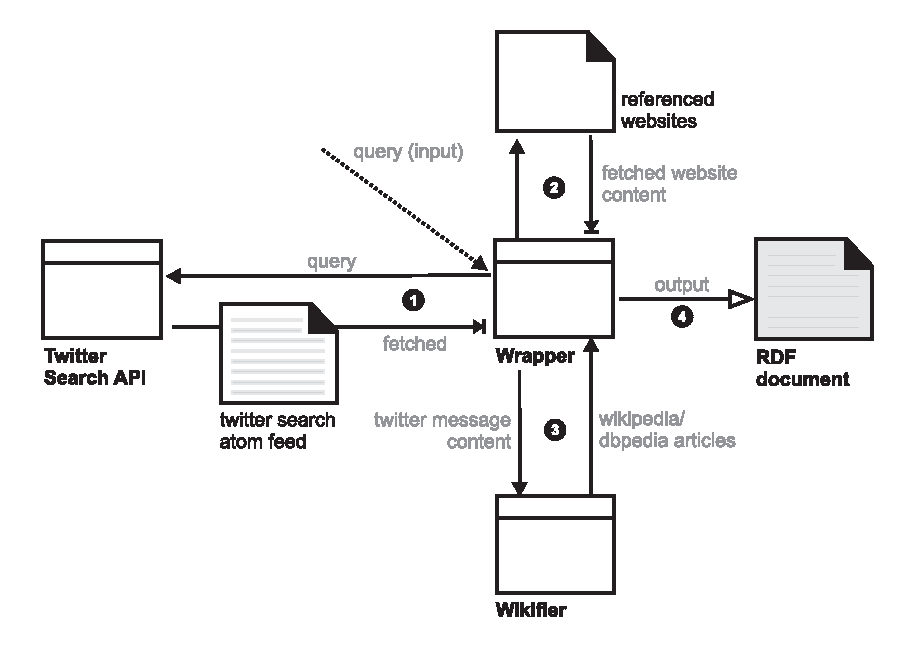
\includegraphics[width=.6\linewidth]{architecture.eps}
  \caption{System architecture}
  \label{fig:arch}
\end{figure}


\section{Experiments and Evaluation}

Trending topics are listed in Table \ref{tbl:terms}.

\begin{table}[ht*]
\centering
\begin{tabular}{ l }
Search term                    \\
\hline
\#s21 \\
Karlsruhe\\
\end{tabular}
\caption{Search terms}\label{tbl:terms}
\end{table}

\section{Conclusion}





\bibliographystyle{abbrv}
\bibliography{bib}

\end{document}
